\documentclass[12pt]{article}
\usepackage[utf8]{inputenc} 
\usepackage{color}
\usepackage{cite}
\usepackage{geometry}                % See geometry.pdf to learn the layout options. There are lots.
%\usepackage{pdflscape}        %single page landscape
                                %mode \begin{landscape} \end{landscape}
\geometry{letterpaper}                   % ... or a4paper or a5paper or ... 
%\usepackage[parfill]{parskip}    % Activate to begin paragraphs with an empty line rather than an indent
\usepackage{multicol} % \begin{multicols}{number of columns} \end{multicols}
\usepackage{graphicx}
\usepackage{amssymb}
\usepackage{Sweave}
\newcommand{\etal}{\textit{et al.}}
\usepackage{hyperref}  %\hyperref[label_name]{''link text''}
                       %\hyperlink{label}{anchor caption}
                       %\hypertarget{label}{link caption}
\linespread{1.5}

\title{Pyrenees, Lebanon Cushion Project}
\author{Michalet, Tousard, Hayek, M.K. Lau}
%\date{}                                           % Activate to display a given date or no date

\begin{document}
\maketitle

\setcounter{tocdepth}{3}  %%activate to number sections
\tableofcontents

\section{Meta}

\begin{verbatim}
    I have now finished to enter the relevés we did with Blaise and
Patrick in Lebanon.
Last time I sent you only the relevés made at a high site and now I
send you the remaining with a low site where we sampled in two grazing
conditions, 4 subsites within fences and 4 outside.
I send you also results of mutivariate analyses I did on the species
composition of all these plots. You will see that different
microhabitats (tight cushions, loose cushions and open) have different
species composition...In some figures plots were gathered depending on
elevation and in another one depending on exposure, which is much better.....
\end{verbatim}

\begin{verbatim}
Hi Matt

This is great that you have time to analyse these dataset.
Yes for sure there is a strong phenotype effect as is telling the
Corespondance Analysis but I guess that your specific network analysis
should precise this tendency.....

Here are the answers to your questions.


Hi Richard (and Patrick and Blaise too!),

Great! I look forward to seeing the Fescue and Genista data as well. I
did a quick run through these data (abundance, richness, compositional
analyses), and the effects of the cushion phenotypes looks very
strong. I should be able to get to a more thorough analysis later this
week. In the meantime, I have a couple of questions (sorry if we've
already gone through this before):

1) What is the difference between the "both" and "afc" data sheets?
You have 6 sheets in the excel file:

- High sites and low sites sheets are the whole dataset (beneficiary
+ environment + cushion traits) of each elevation.

- AFC high sites sheet is the data sheet I prepared to conduct the
correspondance analysis on the high sites only. AFC  (Analyse
Factorielle des Correspondances) in French means CA (Correspondance
Anlysis) in English....

- Both sites sheet is the data sheet including the whole data set
(high and low sites) for the beneficiary species. I prepared this data
sheet for the CA on the whole dataset.

- AFC both sites is the same data sheet but with a filter on the
beneficiary species. I removed all species with a low frequency (below
5 presences in the whole data set). This filter is necessary for the
CA  which results are very influenced by rare species.

2) Are the Loose, Dense and Open "Subsites" indicative of triplets of
samples (i.e. were there Loose, Dense and Open data collected together
in spatial groupings)? It sounds like this is the case, but I wanted
to check. 

In fact there are different open plots for the loose and the dense
cushions plots since they grow in different environmental conditions.
To summarize the design:

You have two elevations (low and high) with a difference in elevation
of approximately 200 meters.

In addition at the low elevation you have a grazing effect.

Then you have the subsites (1 to 5 for the high elevation site and 1
to 4 for the low elevation ungrazed site and 5 to 8 for the low
elevation grazed site).

Those subsites have different exposures (2H, 3H, 4H, 5H, 1L, 3L, 5L,
7L are South and the others are North). Finally when I analysed the
data I realized that exposure had a more important effect on species
composition than elevation,which allows me to conduct a 3 way ANOVA
with exposure, grazing and microhabitats as independent variables but
this a little unbalanced since there are more ungrazed subsites with a
south exposure than with a north exposure (because all high subsites
are ungrazed and 1 of them is in the north for 4 in the south).....

Then at each subsite you have 10 dense-open pairs and 10 loose-open
pairs. The 20 pairs are randomly distributed within a subsite
depending on the environment (convexe vs concave slopes mainly,
respectively). Within a pair the cushion and open plots are very close
to each other (within a meter distance) and in the same environmental
conditions.

Hope this can help.

Cheers

Richard
\end{verbatim}

\begin{verbatim}
Dear Matt

I send you now the complete file for the Pyrénées data that we sampled
Patrick, Blaise and me this summer.
There are 80 relevés with traits, environment and beneficiary species.
Among them are 30 tight cushions (R), 30 loose cushions (D) and 20
intermediate phenotypes (I).
As I told you before there are no open plots at this site since most
of the soil is covered by cushions.
Patrick why is there one cushion line in Yellow (I10)?

So now you have the relevés from Lebanon and Pyrénees (+ Sunset Crater
I guess?) and the only missing are the Sierra Nevada (Spain) but it is
no me who have the field notebooks. I will ask my Spanish
collaborators if they entered yet the data.

Tell me if you need help on these files.

Cheers

Richard
\end{verbatim}

\subsection{Data Summary}
\begin{itemize}
\item Lebanon 
  \begin{itemize}
  \item Two elevations (200 m difference)
  \item Grazing is only at the low elevation
  \item High elevation has 5 subsites
  \item Low elevation has 4 ungrazed and 3 grazed subsites (7 total)
  \item Subsites were spread across N and S aspects (4 on each aspect)
  \item Each subsite has a haphazard sampling of 20 cushion-open pairs
    (10 loose and 10 dense) sampled within 1m of each other
  \end{itemize}
\item Pyrenees
  \begin{itemize}
  \item 30 loose
  \item 30 dense
  \item 20 intermediate
  \item no open
  \item Assume sampled haphazardly, but could be triplets
  \end{itemize}
\end{itemize}

\section{Questions}

\begin{enumerate}
  \begin{enumerate}
  \item Composition
  \item Network structure
    \begin{enumerate}
    \item Bipartite
    \item Unipartite
    \end{enumerate}
  \end{enumerate}
\end{enumerate}

\section{Data}

\begin{Schunk}
\begin{Sinput}
> leb <- read.csv('~/data/pyrenee_lebanon_cushions/plc_2100met1900m_both.csv')
> leb <- list(env=leb[,1:5],com=leb[,-1:-5])
> pyr <- read.csv('~/data/pyrenee_lebanon_cushions/plc_pyrenee_data.csv')
> pyr <- list(env=pyr[,1:15],com=pyr[,-1:-15])
> 
\end{Sinput}
\end{Schunk}

\section{Analyses}

\subsection{Pyr\'{e}n\'{e}es}
%%%Community distance by trait distance
\begin{Schunk}
\begin{Sinput}
> library(vegan)
> library(ecodist)
>                                         #trait distance
> t.d <- dist(pyr$env[,c(7,9:11)])
>                                         #community distance
> com.adj <- apply(pyr$com,2,function(x) x/max(x))
> com.adj <- cbind(com.adj,bca=rep(min(com.adj[com.adj!=0]),nrow(pyr$com)))
> c.d <- vegdist(com.adj)
> mantel(c.d~t.d)
\end{Sinput}
\begin{Soutput}
   mantelr      pval1      pval2      pval3  llim.2.5% ulim.97.5% 
0.08765069 0.00600000 0.99500000 0.01100000 0.05963101 0.13710420 
\end{Soutput}
\begin{Sinput}
> plot(c.d~t.d)
>                                         #permanova
> phenotype <- factor(substr(pyr$env$code,1,1))
> adonis(c.d~phenotype)
\end{Sinput}
\begin{Soutput}
Call:
adonis(formula = c.d ~ phenotype) 

Terms added sequentially (first to last)

          Df SumsOfSqs MeanSqs F.Model      R2 Pr(>F)    
phenotype  2     3.305 1.65265  4.2819 0.10009  0.001 ***
Residuals 77    29.719 0.38596         0.89991           
Total     79    33.024                 1.00000           
---
Signif. codes:  0 ‘***’ 0.001 ‘**’ 0.01 ‘*’ 0.05 ‘.’ 0.1 ‘ ’ 1 
\end{Soutput}
\begin{Sinput}
> 
\end{Sinput}
\end{Schunk}

\begin{Schunk}
\begin{Soutput}
NULL
\end{Soutput}
\begin{Soutput}
NULL
\end{Soutput}
\end{Schunk}
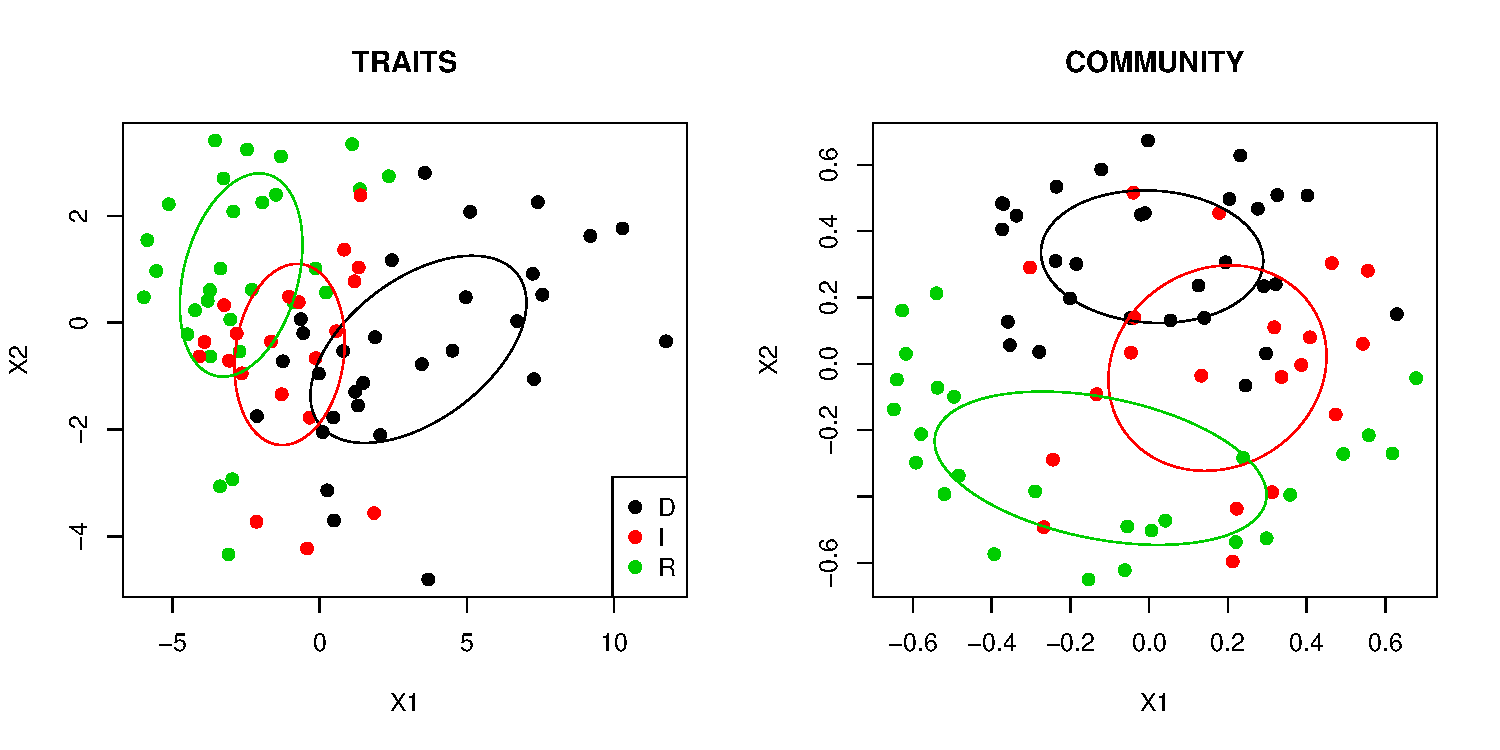
\includegraphics{plc-003}

\end{document}  
